\documentclass[a4paper,10pt]{article}

\usepackage[english]{babel}
\usepackage{graphicx}
\graphicspath{{./figures/}}
\usepackage[colorlinks, linkcolor=black, citecolor=black, urlcolor=black]{hyperref}
\usepackage{geometry}
\geometry{tmargin=3cm, bmargin=2.2cm, lmargin=2.2cm, rmargin=2cm}
\usepackage{todonotes} %Used for the figure placeholders

\begin{document}
\begin{titlepage}
    \newpage
    \thispagestyle{empty}
    \frenchspacing
    \hspace{-0.2cm}
    
\includegraphics[height=3.4cm]{sedes}
    \hspace{0.2cm}
    \rule{0.5pt}{3.4cm}
    \hspace{0.2cm}
    \begin{minipage}[b]{8cm}
        \Large{Katholieke\newline Universiteit\newline Leuven}\smallskip\newline
        \large{}\smallskip\newline
        \textbf{Department of\newline Computer Science}\smallskip
    \end{minipage}
    \hspace{\stretch{1}}
    \vspace*{3.2cm}\vfill
    \begin{center}
        \begin{minipage}[t]{\textwidth}
            \begin{center}
                \LARGE{\rm{\textbf{\uppercase{Document Processing}}\\The
                complete architecture}}\\
                \Large{\rm{Software Architecture (H09B5a and H07Z9a) -- 
                Part 2b}}
            \end{center}
        \end{minipage}
    \end{center}
    \vfill
    \hfill\makebox[8.5cm][l]{%
        \vbox to 7cm{\vfill\noindent
            {\rm \textbf{Thomas Vochten (r0300128)}}\\
            {\rm \textbf{Frederik Goovaerts (r0256551)}}\\[2mm]
            {\rm Academic year 2014--2015}
        }
    }
\end{titlepage}


\tableofcontents
\newpage

\section{Introduction}\label{sec:introduction}

\section{Attribute-driven design documentation}\label{sec:add}
\subsection{Decomposition 1: eDocs System (Av1, P1, UC4, UC5)}
\subsubsection{Module to decompose}
In this (first) run we decompose \texttt{the eDocs System}.

\subsubsection{Selected architectural drivers}
The non-functional drivers for this decomposition are:

\begin{itemize}
    \item \emph{Av1}: Document Generation Failure
    \item \emph{P1}: Document Generation
\end{itemize}

The related functional drivers are:

\begin{itemize}
    \item \emph{UC4}: Generate Payslip
    \item \emph{UC5}: Generate Invoice
\end{itemize}

\paragraph{Rationale}
Both of these non-functional drivers and both use-cases handle the generation of documents by the system. This is one of two core functionalities of the system as a whole, the other being the delivery of said documents. Because they are so important (as also implied by their high priority), makes them both an excellent and cohesive group of drivers for the first run.

\subsubsection{Architectural design}
\paragraph{Raw data queueing for \emph{P1}}
\emph{P1} describes the generation of documents out of raw data. This raw data comes generally comes from a submission subsystem to the generation subsystem. Requiring the generation subsystem to immediately process all received raw data makes for a very strict implementation and possible dropped data when under sudden unforseen load. Due to this, we chose to introduce a component, the \texttt{Raw Data Pool}, which receives the submitted raw data to be processed. The generation subsystem will select raw data out of this pool and mark it as being processed. After a document is generated, the pool is notified that the raw data should be removed. The \texttt{Raw Data Pool} knows of the desired priority scheduling strategy. This strategy allows the pool to sort its contents such that it can always provide the next Raw Data Entry to be generated according to the priority scheduling strategy. The \texttt{Raw Data Pool} is dynamically resizable to store all received raw data entries at any given time. The \texttt{Scheduler Module} (see paragraph ``Recurring load scheduling for P1'') notifies the pool when a large(r) batch of raw data is due, so the pool can expand to accomodate this load. To counter unforseen load, the pool will try to stay under or at half capacity. \todo{Pattern or tactic for this behaviour?} When the pool reaches half capacity, it will signal the document generation subsystem that more parallel generation jobs are necessary to keep the pool from reaching full capacity. When this measure is ineffective, and the pool reaches 75 percent capacity (hereafter called ``critical capacity''), the pool will expand further as necessary to ensure full capacity is never reached. This extra storage can be present on secondary machines, or attained over the network. Whichever solution is the best/cheapest for the eDocs company.

\paragraph{Recurring load scheduling for \emph{P1}}
According to \emph{P1}, the System should anticipate when recurring batches of data are received. For this purpose, a \texttt{Scheduler Module} is introduced. This module knows when a recurring batch is scheduled to be received. A \texttt{Resource Manager} is introduced, whose responsibilies are the allocation of physical space for the \texttt{Raw Data Pool} and signaling the \texttt{Dispatcher Module} for the instantiation and destruction of \texttt{Document Generation Processes} when necessary. The \texttt{Scheduler Module} will signal the \texttt{Resource Manager} how many parallel Document Generation jobs and how much \texttt{Raw Data Pool} capacity should be present, when a recurring batch will be received shortly. This knowledge is introduced/added to the module when a (new) SLA is signed.

\paragraph{Dynamic load anticipation for \emph{P1}}
Apart from recurring batches, the system should provide enough resources (\texttt{Raw Data Pool} capacity and parallel Document Generation jobs) for document generation of non-recurring batches. To regulate the amount of resources available in between recurring batches, a \texttt{Statistics Module} is introduced in the system. This module records the mean amount of processed documents for given time intervals, and supplies the \texttt{Resource Manager} with an estimate of how many document generation resources will be necessary in between recurring batches.

\paragraph{Document Generation Subsystem Structure}
In principle, the Raw Data Pool subcontracts the generation of Documents to several \texttt{Document Generator Processes}. In order to manage the complexity and scalability of this, we propose a \texttt{Raw Data Dispatcher Module}. This module is responsible for knowing which \texttt{Document Generator Processes} are active/instantiated and which Raw Data Entries have been assigned to which \texttt{Processes}. It also records at which time it assigned a specific Entry to which \texttt{Process}. The Raw Data Entry flow is as follows: a \texttt{Document Generator Process} has finished generating a Document according to its assigned Raw Data Entry. The \texttt{Dispatcher Module} temporarily stores the generated Document. The \texttt{Process} simultaneously submits the finished Document to the \texttt{Raw Data Dispatcher Module}, makes the \texttt{Billing Manager} bill the Customer Organization if the Raw Data Entry was from a non-recurring batch, and requests a new Raw Data Entry. The \texttt{Dispatcher Module} submits the finished document to the Document Delivery Subsystem and, when acknowledged, signals the \texttt{Raw Data Pool} that the corresponding Raw Data Entry has been successfully processed and requests the next Raw Data Entry that must be processed. It also deletes the temporarily stores generated Document upon acknowledgement. Upon receipt of the next Raw Data Entry, the \texttt{Dispatcher Module} gives the Entry to the \texttt{Document Generator Process} that initiated the flow and then records the following: the time at which the Entry was assigned, the responsible \texttt{Process} and a reference to the assigned Raw Data Entry. There is also a spare \texttt{Raw Data Dispatcher Module}. This is necessary in case the \texttt{Dispatcher Module} fails (see paragraph ``Raw Data Dispatcher Module Failure Detection and Resolution for \emph{Av1}''). Whenever the active \texttt{Dispatcher Module} records a new Raw Data assignment, it also signals the spare \texttt{Dispatcher Module} to record that assignment as well. The spare \texttt{Dispatcher Module} is aware of the \texttt{Raw Data Pool} and kept up to date on all currently active/instantiated \texttt{Document Generator Processes}. This is done in order to enable the spare \texttt{Dispatcher Module} to assume the responsibilities of the active \texttt{Dispatcher Module} as seamlessly as possible.

\paragraph{Document Generator Process Failure Detection and Resolution for \emph{Av1}}
An individual \texttt{Document Generator Process} may fail. There are two situations in which this may happen: the first (and rather trivial) is when a \texttt{Process} has finished generating a Document and has requested a new Raw Data Entry. When the \texttt{Dispatcher Module} offers a new Raw Data Entry, it is able to detect failure when the \texttt{Process} does not respond. The \texttt{Process} should then be terminated and a new \texttt{Process} instantiated that subsequently starts work on the previously offered Raw Data Entry. The second (and more interesting) case is when a \texttt{Process} fails while generating a Document. In order to counteract Raw Data loss, there is a leasing system in place. The \texttt{Raw Data Dispatcher Module} knows which Raw Data Entries have been assigned to which \texttt{Document Generator Processes}, and each \texttt{Process} has a set lease time during which it should submit the generated Document or renew its lease. A \texttt{Process} may only renew its lease a set amount of times to prevent it from holding on to a Raw Data Entry indefinitely. When a lease has expired, the \texttt{Dispatcher Module} pings the offending \texttt{Process}. If it does not respond with an echo, the \texttt{Process} is marked as failed. If it does respond, the lease is implicitly renewed except if the \texttt{Process} has already reached the maximum amount of lease renewals, in which case it is also marked as failed. As in the first case, when a \texttt{Process} is terminated, a new \texttt{Process} is instantiated and the Raw Data Entry that was previously assigned to the failed \texttt{Process} is then offered to the new \texttt{Process}. 

\paragraph{Raw Data Dispatcher Module Failure Detection and Resolution for \emph{Av1}}
The \texttt{Raw Data Dispatcher Module} may fail. As it is a single point of failure, this issue deserves due consideration. In order to detect failure, there is a \texttt{Dispatcher Supervisor Module}. This module supervises the \texttt{Raw Data Dispatcher Module} by means of a heartbeat. Each time the \texttt{Dispatcher Module} submits a Document to the Document Delivery Subsystem, it also notifies the \texttt{Supervisor}. If there are no Raw Data Entries currently being monitored by the \texttt{Dispatcher Module}, it sends out a notification to the \texttt{Supervisor} at regular intervals that it is still alive, regardless. If the \texttt{Supervisor} has not received a notification from the \texttt{Dispatcher Module} for a set amount of time, it marks the \texttt{Dispatcher Module} as failed. 
As previously mentioned, there is a spare in place that knows which Raw Data Entries have been assigned to which \texttt{Document Generator Processes}. It knows about the \texttt{Raw Data Pool}, the currently active \texttt{Document Generator Processes} and the \texttt{Dispatcher Supervisor Module}. Also, it temporarily stores generated Documents that have yet to be submitted to the Delivery Subsystem and removes those Documents when the currently active \texttt{Dispatcher Module} confirms it has been submitted. When the \texttt{Supervisor} has determined that the currently active \texttt{Dispatcher Module} has failed and has ascertained that the failed \texttt{Dispatcher Module} has terminated, it notifies the spare that it is to assume the responsibilies of newly active \texttt{Dispatcher Module}. The newly active \texttt{Dispatcher Module} then checks the validity of its internal data by contacting the \texttt{Raw Data Pool} and all \texttt{Processes}, in order to ascertain that no events have taken place for the duration of its activation. Also, the newly active \texttt{Dispatcher Module} queries the Delivery Subsystem whether it has already delivered the generated Documents in temporary storage in order to prevent duplicate submissions of generated Documents, removing those that have indeed already been submitted (it is assumed that each Document has a unique identifier). After activation of the now active spare has been completed, the \texttt{Dispatcher Supervisor Module} instantiates a new spare \texttt{Dispatcher Module} and connects it to the currently active \texttt{Dispatcher Module}. The currently active \texttt{Dispatcher Module} then connects the spare to the \texttt{Raw Data Pool} and all currently active \texttt{Document Generator Processes}. Work can then be resumed.
The \texttt{Dispatcher Module} expects an acknowledgement each time it updates the state of the spare. In case there is no acknowledgement, the \texttt{Dispatcher Module} pings the spare. If the spare does not echo in time, it is marked as failed. The \texttt{Dispatcher Module} asks the \texttt{Dispatcher Supervisor Module} for a new spare and shares its state with the new spare. When this is done, work is resumed.

\subsubsection*{Alternatives considered}
\paragraph{Dispatcher Supervisor Module also listening to Document Generator Processes}
It is reasonable to reuse the \texttt{Supervisor} to also listen for the heartbeat of the \texttt{Document Generator Processes}, since this is already its responsibility with regards to the \texttt{Dispatcher Module}. However, this solution would scale poorly and, in addition, the \texttt{Dispatcher Module} has information such that it can more adequately judge whether a certain \texttt{Document Generator Process} has failed.

\paragraph{Dedicated priority scheduling module}
Instead of handing the responsibility of priority scheduling to the \texttt{Raw Data Pool}, it is possible to have another module do this instead. However, it is faster and easier to do this in the \texttt{Raw Data Pool}. Additionally, we do not judge this to lessen the \texttt{Raw Data Pool}'s cohesion and understandability since there are many data structures that also impose an order on the items they store. 

\paragraph{Whether or not to have a \texttt{Raw Data Dispatcher} spare}
In principle, instantiating a new \texttt{Raw Data Dispatcher} and bringing it up to speed can happen quickly by aggregating information from the \texttt{Raw Data Pool}, the currently active \texttt{Document Generator Processes} and the Delivery Subsystem. However, we decided to have a spare as generating documents is one of the core aspects of the system. For this reason, recovering from failure in a timely manner is crucial.

\subsubsection{Instantiation and allocation of functionality}
\paragraph{Decomposition}
Figure \ref{fig:it1-cc_main} shows the components resulting from the decomposition in this run. Extra attention is required concerning the \texttt{Dispatcher Module} and \texttt{Spare Dispatcher Module}. These components are actually two instances of the same dispatching component. Therefore, they provide and require the same interfaces. But depending on their run-time role, i.e. primary or standby dispatcher (cf. the decisions concerning \emph{Av1} above), a specific set of these is activated. This is indicated by having both component instances provide and require the same interfaces, but differing the connections between components dependent on the role of the instance. Additional notes are added to the diagram where deemed necessary.

\subparagraph{Dispatcher Module}
Responsible for serving the \texttt{Document Generator Processes} with new Raw Data Entries when asked. Also responsible for recording the leases on each served Entry, and monitoring these leases to ping \texttt{Document Generator Processes} when leases expire. When a \texttt{Generator Process} has failed, it removes the failed \texttt{Process} and instantiates a new one. It also instantiates and destroys \texttt{Generator Processes} when instructed to by the \texttt{Resource Manager}. Receives generated Documents form the \texttt{Generator Processes} and submits these to the delivery system (\texttt{Other Functionality}). Signals the Billing Manager when a document from a non-recurring Raw Data batch has been processed so that the Customer Organization can be billed. Also responsible for sending a Heartbeat pulse to the \texttt{Dispatcher Supervisor}, piggybacked on a document submission whenever possible. At every change to its internal data, the \texttt{Dispatcher Module} should send this change to the \texttt{Spare Dispatcher Module} to keep their states consistent. When the \texttt{Spare Dispatcher Module} does not acknowledge the changes, it should be pinged by the \texttt{Dispatcher Module}, and if it has failed, the latter should request a new \texttt{Spare Dispatcher Module} from the \texttt{Dispatcher Supervisor}.

\subparagraph{Raw Data Pool}
Responsible for storing Raw Data Entries that have not yet been processed. Also responsible for sorting/scheduling these Entries according to deadline priorities, and recording which Entries are currently being processed. Submits statistics about its capacity usage to the \texttt{Statistics Module}.

\subparagraph{Document Generator Process}
Responsible for generating Documents out of Raw Data Entries. Queries the \texttt{Dispatcher Module} for a new Entry when it has finished generating a document along with submitting the generated document back to the \texttt{Dispatcher Module}. Requests the Template for use with its Raw Data (\texttt{Other Functionality}), and when a PDF has been generated, hands this to the System for signing (\texttt{Other Functionality}) when necessary (E.g. invoices), before submission.

\subparagraph{Dispatcher Supervisor}
Responsible for listening to the heartbeat of the \texttt{Dispatcher Module}. If the heartbeat fails, it should activate the \texttt{Spare Dispatcher Module} and terminate the active \texttt{Dispatcher Module}. Should the \texttt{Dispatcher Module} request a new \texttt{Spare Dispatcher Module}, it terminates the current \texttt{Spare Dispatcher Module} and instantiates a new one and informs the \texttt{Dispatcher Module} about it.

\subparagraph{Spare Dispatcher Module}
Here, the internal data of the \texttt{Dispatcher Module} is duplicated so that it can assume the responsibilities of the \texttt{Dispatcher Module} upon failure. When its state is updated, it should send an acknowledgement to the \texttt{Dispatcher Module}. It must also respond to pings from the \texttt{Dispatcher Module}.

\subparagraph{Submission Subsystem}
To be decomposed in a future run. It accepts Raw Data Batches from the Customer Organisation and hands it to the Raw Data Pool.

\subparagraph{Statistics Module}
Responsible for accepting data statistics for the \texttt{Raw Data Pool} and interpreting these. It also signals the \texttt{Resource Manager} about the projected resources it should allocate for document generation of non-recurring batches.

\subparagraph{Scheduler Module}
Manages and receives the schedule of recurring Raw Data batches. If a batch is imminent, it should the \texttt{Resource Manager} about the resources it should allocate for document generation of the recurring batch(es).

\subparagraph{Resource Manager}
Responsible for allocating adequate space in the \texttt{Raw Data Pool} and giving guidelines to the \texttt{Dispatcher Module} as to how many \texttt{Document Generator Process}es it would be appropriate to maintain. It should do this based on information it receives from the \texttt{Statistics Module} and the \texttt{Scheduler Module}.

\subparagraph{Billing Manager}
Responsible for managing billing information for each Customer Organization. It must be possible to bill Customer Organizations for both recurring batches and non-recurring batches. The \texttt{Billing Manager} must supply billing information on Customer Organizations on demand.

\subparagraph{Other Functionality}
Encapsulates requirements not tackled in this run and which cannot be
assigned to other introduced components.

\begin{figure}[!htp]
    \centering
    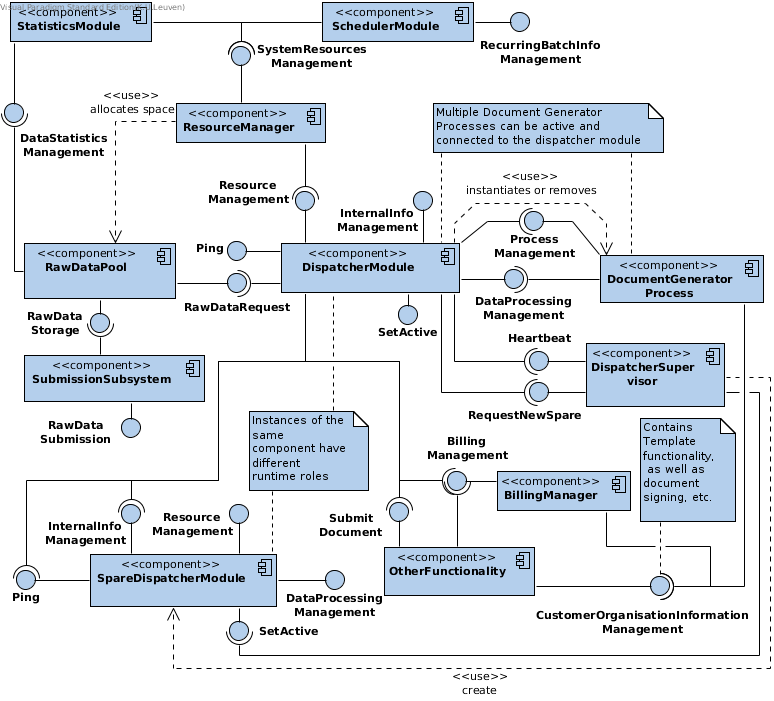
\includegraphics[width=\textwidth]{comp_diag_1.png}
    %\missingfigure[figwidth=0.8\textwidth]{Component-and-connector diagram}
    \caption{Component-and-connector diagram of this decomposition.}\label{fig:it1-cc_main}
\end{figure}

\paragraph{Behaviour}
Figure \ref{fig:it1-seq_aspect1} illustrates the standard flow of document generation in the system. This flow is initiated by the \texttt{Generator Processes} themselves. When new Raw Data is requested and none is found, \texttt{Generator Processes} go into standby. When the \texttt{Dispatcher Module} is notified of new data being available, it can reactivate the \texttt{Generator Processes}.

\begin{figure}[!htp]
    \centering
    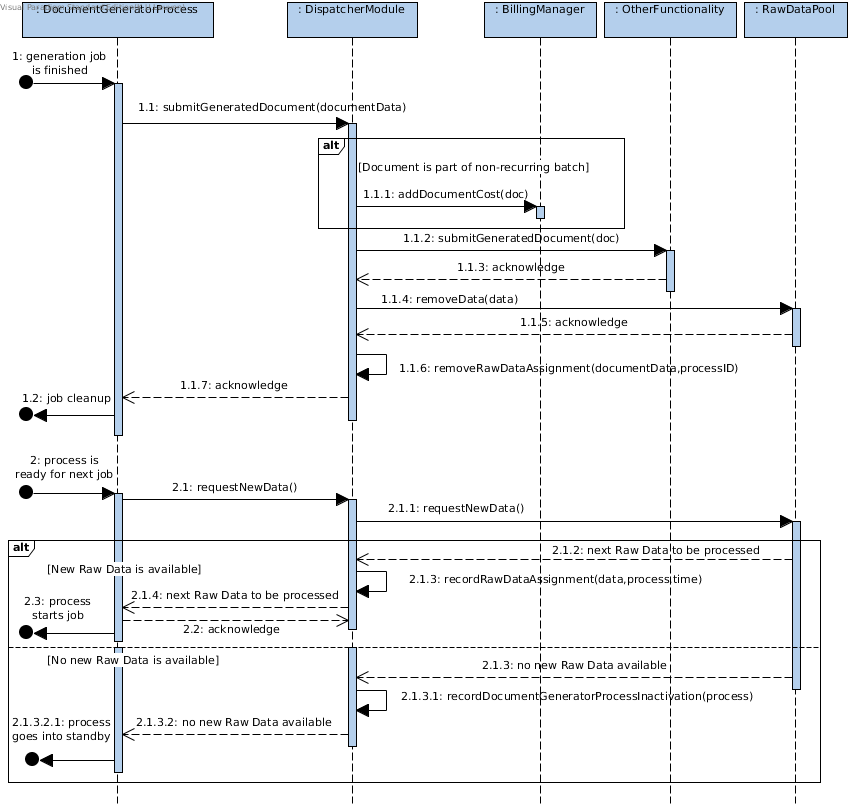
\includegraphics[width=\textwidth]{seq_diag_1_-_doc_gen.png}
    %\missingfigure[figwidth=0.8\textwidth]{Sequence diagram}
    \caption{Sequence diagram illustrating the flow of document generation.}\label{fig:it1-seq_aspect1}
\end{figure}

\paragraph{Deployment}
Figure \ref{fig:it1-depl_main} show the mapping of architectural components on physical nodes.
The entry main entry point and accompanying storage components of the system are gathered on the \texttt{RawDataHandlingNode}, since these work together closely and depend on eachother. Also, they are a cohesive part of the system regarding behaviour. The \texttt{Dispatcher Supervisor} and both \texttt{Dispatcher Module}s are key components in the system, being the central focus of behaviour. They each have their own node, being essential parts, so simultaneous failure is less likely. The \texttt{Document Generator Processes} are mapped to their own dedicated nodes because they are work processes and specialised powerful nodes can be provided to them. They can be distributed along multiple of these nodes so when a lot of work is done, failure of one work node doesn't bring the system to a halt. The remaining functionality of the system, most of which is used later than the selected drivers, is mapped to an OtherFunctionalityNode, which is to be decomposed later.

\begin{figure}[!htp]
    \centering
    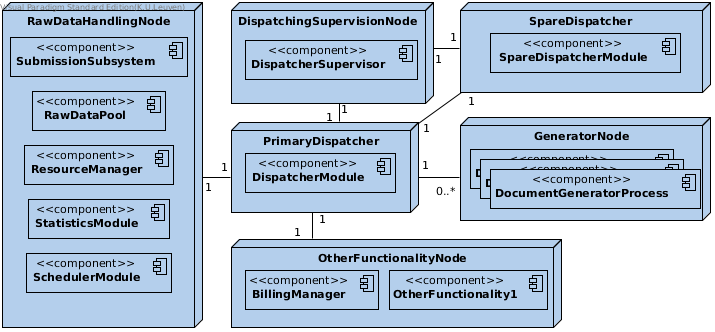
\includegraphics[width=0.8\textwidth]{depl_diag_1.png}
    %\missingfigure[figwidth=0.8\textwidth]{Deployment diagram}
    \caption{Deployment diagram of this decomposition.}\label{fig:it1-depl_main}
\end{figure}

\subsubsection{Interfaces for child modules}
\subsubsection*{Dispatcher Module}
\begin{itemize}
    \item DataProcessingManagement
    \begin{itemize}
        \item \texttt{RawDataEntry requestNewData()}
        \begin{itemize}
            \item Effect: Supply a new Raw Data Entry. May be an empty entry if no Raw Data Entry is available.
        \end{itemize}
        
        \item \texttt{void submitGeneratedDocument(DocumentData generated)} throws InvalidDocumentDataException
        \begin{itemize}
            \item Effect: Accept a generated document so that it may be delivered and the Customer Organization billed if appropriate.
            \item Exceptions:
            \begin{itemize}
            	\item InvalidDocumentDataException: The DocumentData argument is badly structured
            \end{itemize}
        \end{itemize}
    \end{itemize}
	\item Ping
	\begin{itemize}
		\item \texttt{Echo ping()}
		\begin{itemize}
			\item Effect: Returns an Echo to reassure the caller that the callee is still available. 
			\item Exceptions: None
		\end{itemize}
	\end{itemize}
\end{itemize}

\begin{itemize}
	\item ResourceManagement
	\begin{itemize}
		\item \texttt{void notify(ResourceGuidelineReport report)}
		\begin{itemize}
			\item Effect: Supply information that is relevant to how many \texttt{Document Generator Process}es the \texttt{Dispatcher Module} should maintain. The \texttt{Dispatcher Module} returns immediately and thereafter takes appropriate actions (e.g. instantiate new \texttt{Document Generator Process}es).
			\item Exceptions: None
		\end{itemize}
	\end{itemize}
\end{itemize}

\todo{Verification of data when spare becomes active}
\begin{itemize}
	\item InternalInfoManagement
	\begin{itemize}
		\item \texttt{void recordNewDocumentGeneratorProcess(DocumentGeneratorProcessID id)}
		\begin{itemize}
			\item Effect: Records the identifier of a new \texttt{DocumentGeneratorProcess}. No effect if the identifier has been supplied previously.
			\item Exceptions: None
		\end{itemize}
		
		\item \texttt{void recordDocumentGeneratorProcessRemoval(DocumentGeneratorProcessID id)}
		\begin{itemize}
			\item Effect: Records that the \texttt{DocumentGeneratorProcess} with the specified identifier has been removed from the system. No effect if the identifier was not supplied earlier through \texttt{recordNewDocumentGeneratorProcess(DocumentGeneratorProcessID)}.
			\item Exceptions: None
		\end{itemize}
		
		\item \texttt{void recordRawDataAssignment(RawDataEntry entry, DocumentGeneratorProcessID id}
		\begin{itemize}
			\item Effect: Records that the specified Raw Data Entry has been assigned to the specified \texttt{DocumentGeneratorProcess}. No effect if that pair has already been recorded.
			\item Exceptions: None
		\end{itemize}
		
		\item \texttt{void removeRawDataAssignment(RawDataEntry entry, DocumentGeneratorProcessID id}
		\begin{itemize}
			\item Effect: Removes the assignment of the specified Raw Data Entry to the specified \texttt{DocumentGeneratorProcess}. No effect if that pair is not recorded.
			\item Exceptions: None
		\end{itemize}
		
		\item \texttt{void recordGeneratedDocument(DocumentData generated)}
		\begin{itemize}
			\item Effect: Stores the supplied generated document in secondary storage.
			\item Exceptions: None
		\end{itemize}
		
		\item \texttt{void removeGeneratedDocument(DocumentDataID id)} throws DocumentNotFoundException
		\begin{itemize}
			\item Effect: Deletes the corresponding DocumentData from secondary storage.
			\item Exceptions:
			\begin{itemize}
				\item DocumentNotFoundException: No corresponding DocumentData exists in storage.
			\end{itemize}
		\end{itemize}
	\end{itemize}
\end{itemize}

\begin{itemize}
	\item SetActive
	\begin{itemize}
		\item \texttt{void activate} throws AlreadyActiveException
		\begin{itemize}
			\item Effect: 
			\begin{itemize}
				\item Looks up and assumes control of all \texttt{DocumentGeneratorProcess}es it has an identifier of.
				\item Verifies the correctness of its internal state by contacting the \texttt{RawDataPool} (to verify which Raw Data Entries have been marked as work in progress), \texttt{DocumentGeneratorProcess}es (to verify assignments of Raw Data Entries to \texttt{Processes}) and \texttt{OtherFunctionality} (to verify which generated documents it has in storage have already been delivered.
				\item Requests a new spare \texttt{DispatcherModule} from the \texttt{DispatcherSupervisor}
				\item Copies its state to the new spare
				\item Returns and resumes normal operation
			\end{itemize}
			\item Exceptions: 
			\begin{itemize}
				\item AlreadyActiveException: This \texttt{DispatcherModule} is the active \texttt{DispatcherModule}
			\end{itemize}
		\end{itemize}
	\end{itemize}
\end{itemize}

\subsubsection*{DocumentGeneratorProcess}
\begin{itemize}
	\item ProcessManagement
	\begin{itemize}
		\item \texttt{ProcessStatusReport getStatusReport(RawDataEntryID id)}
		\begin{itemize}
			\item Effect: Indicates through the returned object whether it is working on the specified Raw Data Entry and if it has finished or not
			\item Exceptions: None
		\end{itemize}
		
		\item \texttt{Echo ping()}
		\begin{itemize}
			\item Effect: Returns an Echo to reassure the caller that the callee is still available.
			\item Exceptions: None
		\end{itemize}
		
		\item \texttt{void assignRawData(RawDataEntry entry)} throws NotIdleException
		\begin{itemize}
			\item Effect: Assigns the specified RawDataEntry to this \texttt{DocumentGeneratorProcess}
			\item Exceptions: 
			\begin{itemize}
				\item NotIdleException: This \texttt{DocumentGeneratorProcess} is already working on another RawDataEntry.
			\end{itemize}
		\end{itemize}
		
		\item \texttt{DocumentData getGeneratedDocument()} throws NoDocumentDataAvailableException
		\begin{itemize}
			\item Effect: Supplies the document generated from its assigned Raw Data Entry
			\item Exceptions: 
			\begin{itemize}
				\item TypeOfException: Document generation has not yet been finished or no RawDataEntry has been assigned.
			\end{itemize}
		\end{itemize}
	\end{itemize}
\end{itemize}

\subsubsection*{RawDataPool}
\begin{itemize}
	\item GetNextRawData
	\begin{itemize}
		\item \texttt{RawDataEntry requestNewData()}
		\begin{itemize}
			\item Effect: Supplies the next RawDataEntry that should be processed. If no Entry is available, an empty Entry is returned.
			\item Exceptions: None
		\end{itemize}
		
		\item \texttt{PoolDataReport getDataReport()}
		\begin{itemize}
			\item Effect: Supplies information about which RawDataEntry entries have been marked as work in progress.
			\item Exceptions: None
		\end{itemize}
		
		\item \texttt{void removeData(RawDataEntryID id)} throws NoSuchRawDataEntryException
		\begin{itemize}
			\item Effect: Removes the corresponding RawDataEntry from the pool.
			\item Exceptions: 
			\begin{itemize}
				\item NoSuchRawDataEntryException: There is no corresponding RawDataEntry.
			\end{itemize}
		\end{itemize}
	\end{itemize}
\end{itemize}

\begin{itemize}
	\item SubmitDataForProcessing
	\begin{itemize}
		\item \texttt{void submitRawDataBatch(RawDataBatch data)}
		\begin{itemize}
			\item Effect: Adds the RawData in the specified RawDataBatch to the pool. A unique identifier is generated for each RawData and the resulting RawDataEntry entries are scheduled according to the scheduling policy.
			\item Exceptions: None
		\end{itemize}
	\end{itemize}
\end{itemize}

\subsubsection*{DispatcherSupervisor}
\begin{itemize}
	\item Heartbeat
	\begin{itemize}
		\item \texttt{void supplyHeartbeat()} throws TypeOfException
		\begin{itemize}
			\item Effect: Records a heartbeat from the supervised component.
			\item Exceptions: None
		\end{itemize}
	\end{itemize}
\end{itemize}

\begin{itemize}
	\item RequestNewSpare
	\begin{itemize}
		\item \texttt{DispatcherID requestNewSpareDispatcher()}
		\begin{itemize}
			\item Effect: Initialises a new spare \texttt{DispatcherModule} and generates an ID for it such that callee can find the new spare.
			\item Exceptions: None
		\end{itemize}
	\end{itemize}
\end{itemize}

\subsubsection*{StatisticsModule}
\begin{itemize}
	\item DataStatisticsManagement
	\begin{itemize}
		\item \texttt{void deliver(StatisticsReport report)}
		\begin{itemize}
			\item Effect: Integrates the information supplied by the given report into its own information (e.g. mean pool capacity during a certain period in a certain month).
			\item Exceptions: None
		\end{itemize}
	\end{itemize}
\end{itemize}

\subsubsection*{SchedulerModule}
\begin{itemize}
	\item RecurringBatchInfoManagement
	\begin{itemize}
		\item \texttt{void recordRecurringBatch(Date date, int maxAmount)}
		\begin{itemize}
			\item Effect: Records that a batch with the specified maximal amount is expected at the specified date.
			\item Exceptions: None
		\end{itemize}
		
		\item \texttt{void deleteRecurringBatch(Date date, int maxAmount)}
		\begin{itemize}
			\item Effect: Records that a batch on the specified date with the specified maximal amount will no longer occur.
			\item Exceptions: None
		\end{itemize}
	\end{itemize}
\end{itemize}

\subsubsection*{SubmissionSubsystem}
\begin{itemize}
	\item SubmitRawDataBatch
	\begin{itemize}
		\item \texttt{void submitRawDataBatch(RawDataBatch batch)}
		\begin{itemize}
			\item Effect: Submits the given RawDataBatch for processing.
			\item Exceptions: None
		\end{itemize}
	\end{itemize}
\end{itemize}

\subsubsection*{BillingManager}
\begin{itemize}
	\item BillingManagement
	\begin{itemize}
		\item \texttt{void billCustomer(RawDataEntry entry)}
		\begin{itemize}
			\item Effect: Extracts the required information to bill the Customer Organization for generation of the document from the RawDataEntry (e.g. document type, priority) on the one hand and from Customer Organization information stored elsewhere in the system on the other hand and records a new billing for the Customer Organization.
			\item Exceptions: None
		\end{itemize}
	\end{itemize}
\end{itemize}

\subsubsection*{OtherFunctionality}
\begin{itemize}
	\item SubmitDocument
	\begin{itemize}
		\item \texttt{void submitDocument(DocumentData data)}
		\begin{itemize}
			\item Effect: Initiates the submission process for the specified generated document
			\item Exceptions: None
		\end{itemize}
		
		\item \texttt{boolean getDocumentSubmissionReport(DocumentDataID data)}
		\begin{itemize}
			\item Effect: Indicates whether the generated document corresponding to the given DocumentDataID has already been delivered.
			\item Exceptions: None
		\end{itemize}
	\end{itemize}
\end{itemize}

\subsubsection{Data type definitions}
Describe per complex data type used in the interfaces what it represents.

\paragraph{returnType} This data element represents X.

\paragraph{ParamType} This data element represents Y.

\subsubsection{Verify and refine}
This section describes per component which (parts of) the remaining requirements it is responsible for. If requirements are split, a letter is added to its name (e.g. Av1a) to indicate that the component will only satisfy a part of the original requirement. If requirements are split, it will also be indicated what part of the original requirement each new requirement contains. If new derived requirements are introduced they will receive a new identifier and are marked as a new requirement.

\paragraph{OtherFunctionality}
\begin{itemize}
    \item \emph{UC1}: Log in
    \item \emph{UC2}: Log out
    \item \emph{UC6}: Deliver document via e-mail
    \item \emph{UC7}: Notify of e-mail delivery failure
    \item \emph{UC8}: Deliver document via postal mail
    \item \emph{UC9}: Deliver invoice via Zoomit
    \item \emph{UC10}: Confirm document delivery (Zoomit)
    \item \emph{UC11}: Deliver document via personal document store
    \item \emph{UC12}: Consult personal document store
    \item \emph{UC13}: Search documents in personal document store
    \item \emph{UC14}: Consult document in personal document store
    \item \emph{UC15}: Download document via unique link
    \item \emph{UC16}: Register to personal document store
    \item \emph{UC17}: Unregister from personal document store
    \item \emph{UC18}: Register customer organization
    \item \emph{UC19}: Unregister customer organization
    \item \emph{UC20}: Update document template
    \item \emph{UC21a}: Consult status of all document processing jobs\\
    Handling the (visual) interfacing with the user. Determining the finished jobs.
    \item \emph{UC22}: Notify customer administrator
    \item \emph{Av2}: Personal document storage failure 
    \item \emph{Av3}: Zoomit failure
    \item \emph{P2}: Document lookups
    \item \emph{P3a}: Status overview for customer administrators\\
    Handling the flow of this requirement and the overal processing of the status reports in a timely fashion.
    \item \emph{M1a}: New type of document: bank statements\\
    The delivery and template handling for the new document.
    \item \emph{M2}: Multiple print \& postal services
    \item \emph{M3}: Dynamic selection of the cheapest of print \& postal services
\end{itemize}

\paragraph{SubmissionSubsystem}
\begin{itemize}
    \item \emph{UC3}: Initiate document processing
    \item \emph{M1b}: New type of document: bank statements\\
    Being able to receive and verify the integrity of Raw Data for the new type of document.
\end{itemize}

\paragraph{RawDataPool}
\begin{itemize}
    \item \emph{UC21b}: Consult status of all document processing jobs\\
    Determining the unfinished and currently processing jobs.
    \item \emph{P3b}: Status overview for customer administrators\\
    Calculating and delivering information about all unfinished and currently processing jobs for a certain \texttt{Customer Organisation} in a timely fashion.
\end{itemize}

\paragraph{DocumentGenerationProcess}
\begin{itemize}
    \item \emph{M1c}: New type of document: bank statements\\
    Being able to generate documents of the new type with the accompanying new template.
\end{itemize}

\subsection{Decomposition 2: Module (drivers)}
\subsubsection{Module to decompose}
\subsubsection{Selected architectural drivers}
\subsubsection{Architectural design}
\subsubsection{Instantiation and allocation of functionality}
\subsubsection{Interfaces for child modules}
\subsubsection{Data type definitions}
\subsubsection{Verify and refine}

\subsection{Decomposition 3: Module (drivers)}
\subsubsection{Module to decompose}
\subsubsection{Selected architectural drivers}
\subsubsection{Architectural design}
\subsubsection{Instantiation and allocation of functionality}
\subsubsection{Interfaces for child modules}
\subsubsection{Data type definitions}
\subsubsection{Verify and refine}

\section{Resulting partial architecture}\label{sec:architecture}
This section provides an over of the architecture constructed through ADD\@.

\subsection{Context diagram}
This subsection discusses the context diagram.

\begin{figure}[!htp]
    \centering
    %\includegraphics[width=0.8\textwidth]{}
    \missingfigure[figwidth=0.8\textwidth]{Context diagram for component-and-
        connector view.}
    \caption{Context diagram for the component-and-connector view.
        }\label{fig:cc_context}
\end{figure}

\subsection{Component-and-connector view}
A short discussion of the component-and-connector view with the key
decompositions if any.

\begin{figure}[!htp]
    \centering
    %\includegraphics[width=0.8\textwidth]{}
    \missingfigure[figwidth=0.8\textwidth]{Component-and-connector diagram}
    \caption{Primary diagram for the component-and-connector view.
        }\label{fig:cc_main}
\end{figure}

\begin{figure}[!htp]
    \centering
    %\includegraphics[width=0.8\textwidth]{}
    \missingfigure[figwidth=0.8\textwidth]{Key decomposition}
    \caption{Decomposition of a component shown in Figure~\ref{fig:cc_main}
        }\label{fig:decomp_decomp1}
\end{figure}

\subsection{Deployment view}
A short discussion of the allocation of components to physical nodes based on a
context diagram and a deployment diagram.

\begin{figure}[!htp]
    \centering
    %\includegraphics[width=0.8\textwidth]{}
    \missingfigure[figwidth=0.8\textwidth]{Context diagram for the allocation
        view.}
    \caption{Context diagram for the allocation view.}\label{fig:depl_context}
\end{figure}

\begin{figure}[!htp]
    \centering
    %\includegraphics[width=0.8\textwidth]{}
    \missingfigure[figwidth=0.8\textwidth]{Deployment diagram}
    \caption{Primary diagram for the allocation view.}\label{fig:depl_main}
\end{figure}

\end{document}
